% Options for packages loaded elsewhere
\PassOptionsToPackage{unicode}{hyperref}
\PassOptionsToPackage{hyphens}{url}
%
\documentclass[
]{book}
\usepackage{lmodern}
\usepackage{amssymb,amsmath}
\usepackage{ifxetex,ifluatex}
\ifnum 0\ifxetex 1\fi\ifluatex 1\fi=0 % if pdftex
  \usepackage[T1]{fontenc}
  \usepackage[utf8]{inputenc}
  \usepackage{textcomp} % provide euro and other symbols
\else % if luatex or xetex
  \usepackage{unicode-math}
  \defaultfontfeatures{Scale=MatchLowercase}
  \defaultfontfeatures[\rmfamily]{Ligatures=TeX,Scale=1}
\fi
% Use upquote if available, for straight quotes in verbatim environments
\IfFileExists{upquote.sty}{\usepackage{upquote}}{}
\IfFileExists{microtype.sty}{% use microtype if available
  \usepackage[]{microtype}
  \UseMicrotypeSet[protrusion]{basicmath} % disable protrusion for tt fonts
}{}
\makeatletter
\@ifundefined{KOMAClassName}{% if non-KOMA class
  \IfFileExists{parskip.sty}{%
    \usepackage{parskip}
  }{% else
    \setlength{\parindent}{0pt}
    \setlength{\parskip}{6pt plus 2pt minus 1pt}}
}{% if KOMA class
  \KOMAoptions{parskip=half}}
\makeatother
\usepackage{xcolor}
\IfFileExists{xurl.sty}{\usepackage{xurl}}{} % add URL line breaks if available
\IfFileExists{bookmark.sty}{\usepackage{bookmark}}{\usepackage{hyperref}}
\hypersetup{
  pdftitle={UC Mission Binder},
  pdfauthor={UC Center of Excellence on UAS Safety},
  hidelinks,
  pdfcreator={LaTeX via pandoc}}
\urlstyle{same} % disable monospaced font for URLs
\usepackage{longtable,booktabs}
% Correct order of tables after \paragraph or \subparagraph
\usepackage{etoolbox}
\makeatletter
\patchcmd\longtable{\par}{\if@noskipsec\mbox{}\fi\par}{}{}
\makeatother
% Allow footnotes in longtable head/foot
\IfFileExists{footnotehyper.sty}{\usepackage{footnotehyper}}{\usepackage{footnote}}
\makesavenoteenv{longtable}
\usepackage{graphicx,grffile}
\makeatletter
\def\maxwidth{\ifdim\Gin@nat@width>\linewidth\linewidth\else\Gin@nat@width\fi}
\def\maxheight{\ifdim\Gin@nat@height>\textheight\textheight\else\Gin@nat@height\fi}
\makeatother
% Scale images if necessary, so that they will not overflow the page
% margins by default, and it is still possible to overwrite the defaults
% using explicit options in \includegraphics[width, height, ...]{}
\setkeys{Gin}{width=\maxwidth,height=\maxheight,keepaspectratio}
% Set default figure placement to htbp
\makeatletter
\def\fps@figure{htbp}
\makeatother
\setlength{\emergencystretch}{3em} % prevent overfull lines
\providecommand{\tightlist}{%
  \setlength{\itemsep}{0pt}\setlength{\parskip}{0pt}}
\setcounter{secnumdepth}{-\maxdimen} % remove section numbering
\usepackage{booktabs}
\usepackage[left=2cm,right=2cm,top=2cm,bottom=2cm]{geometry}

\usepackage{fancyhdr}
\pagestyle{plain}



\let\origdoublepage\cleardoublepage
\newcommand{\clearemptydoublepage}{\clearpage{\pagestyle{empty}\origdoublepage}}
\let\cleardoublepage\clearemptydoublepage
\makeatletter
\renewcommand\part{%
   \if@openright
     \cleardoublepage
   \else
     \clearpage
   \fi
   \thispagestyle{empty}%
   \if@twocolumn
     \onecolumn
     \@tempswatrue
   \else
     \@tempswafalse
   \fi
   \null\vfil
   \secdef\@part\@spart}
\makeatother
\renewcommand\thepage{}

\let\oldmaketitle\maketitle
\AtBeginDocument{\let\maketitle\relax}
\AtBeginDocument{\let\tableofcontents\relax}
\usepackage[]{natbib}
\bibliographystyle{apalike}

\title{UC Mission Binder}
\author{UC Center of Excellence on UAS Safety}
\date{2020-10-07}

\begin{document}
\maketitle

\thispagestyle{empty}
\begin{center}
\vspace*{9em}
{\Huge UC Mission Binder}\\
\vspace*{9em}
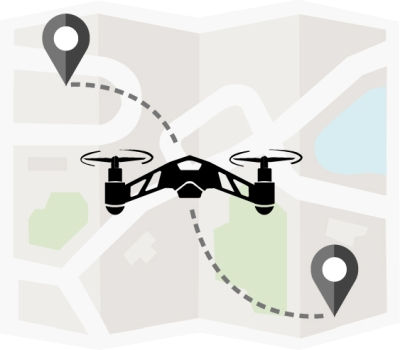
\includegraphics{cover.jpg}\\
\vspace*{9em}
{\huge 

Mission: \hrulefill

Dates: \hrulefill

Flight Crew: \hrulefill

}
\vspace*{9em}
\end{center}

\let\maketitle\oldmaketitle

{
\setcounter{tocdepth}{1}
\tableofcontents
}
\hypertarget{document-summary}{%
\chapter*{Document Summary}\label{document-summary}}
\addcontentsline{toc}{chapter}{Document Summary}

This document serves as a template for the assembly of a UAS Mission Binder for UAS operations within the University of California System. It provides a set of standard guidance and supporting templates that the Flight Crew may utilize.

\begin{center}\rule{0.5\linewidth}{0.5pt}\end{center}

\hypertarget{mission-binder-requirements}{%
\section*{Mission Binder Requirements}\label{mission-binder-requirements}}
\addcontentsline{toc}{section}{Mission Binder Requirements}

\begin{itemize}
\tightlist
\item
  UAS Policy: \href{https://policy.ucop.edu/doc/3500671/Drone}{link}
\item
  UC Operation Manuals: \href{https://ucdrones.github.io/ch-user-guides.html}{link}
\item
  UC Standard Guidance
\item
  Mission Documentation (Have available online or printed)

  \begin{itemize}
  \tightlist
  \item
    UC Drone Approval
  \item
    Documented Procedures
  \item
    Risk Assessment
  \item
    Emergency Action Plans \href{http://ucdrones.github.io/library/emergency_procedure_checklists.docx}{Template Here}
  \end{itemize}
\item
  Remote Pilot Certificate
\item
  UAS Registration Certificate
\item
  Airspace Authorization or Waiver Documentation
\end{itemize}

\hypertarget{ch-docs}{%
\chapter{UC Documentation}\label{ch-docs}}

\hypertarget{uc-policy}{%
\section{UC Policy}\label{uc-policy}}

The UC UAS Policy can be found here: \url{https://policy.ucop.edu/doc/3500671/Drone}

\hypertarget{uc-uas-operations-manuals}{%
\section{UC UAS Operations Manuals}\label{uc-uas-operations-manuals}}

The UC UAS Operations Manuals can be found at \url{https://ucdrones.github.io}

\begin{itemize}
\tightlist
\item
  New User Guide: \url{https://ucdrones.github.io/New_User_Guide/}
\item
  Standard Operations Procedures - Advanced Operations: \url{https://ucdrones.github.io/Advanced_SOP/}
\end{itemize}

\hypertarget{part-uc-operating-standards}{%
\part{UC Operating Standards}\label{part-uc-operating-standards}}

\hypertarget{standard-guidance}{%
\chapter{Standard Guidance}\label{standard-guidance}}

\begin{itemize}
\tightlist
\item
  All UAS activity must establish a buffer or safe-zone between the Unmanned Aircraft and any non-participating persons or sensitive locations.

  \begin{itemize}
  \tightlist
  \item
    A good rule-of-thumb is to maintain a buffer or safe-zone of roughly \(\frac{1}{4}^{th}\) of the flight altitude.
  \end{itemize}
\item
  Visual Observers and supporting ground crew should be utilized when available.

  \begin{itemize}
  \tightlist
  \item
    Supporting ground crew should assist in ensuring safety to all non-participating persons.
  \end{itemize}
\item
  All members of the flight crew must be conspicuous and wear professional, identifying apparel such as university-branded hats, shirts or lanyards with IDs.
\item
  High visibility reflective vests must be worn when operating near roads or in parking lots.\\
\item
  When operating in fenced areas, operate exclusively within the fenced areas unless there is sufficient visibility on the other side to ensure safety to non-participants.
\item
  Never fly in areas where UAS activity is prohibited or restricted.
\item
  Always be a good neighbor and ensure that your UAS activity is not disruptive to other authorized activities.
\end{itemize}

\begin{figure}

{\centering 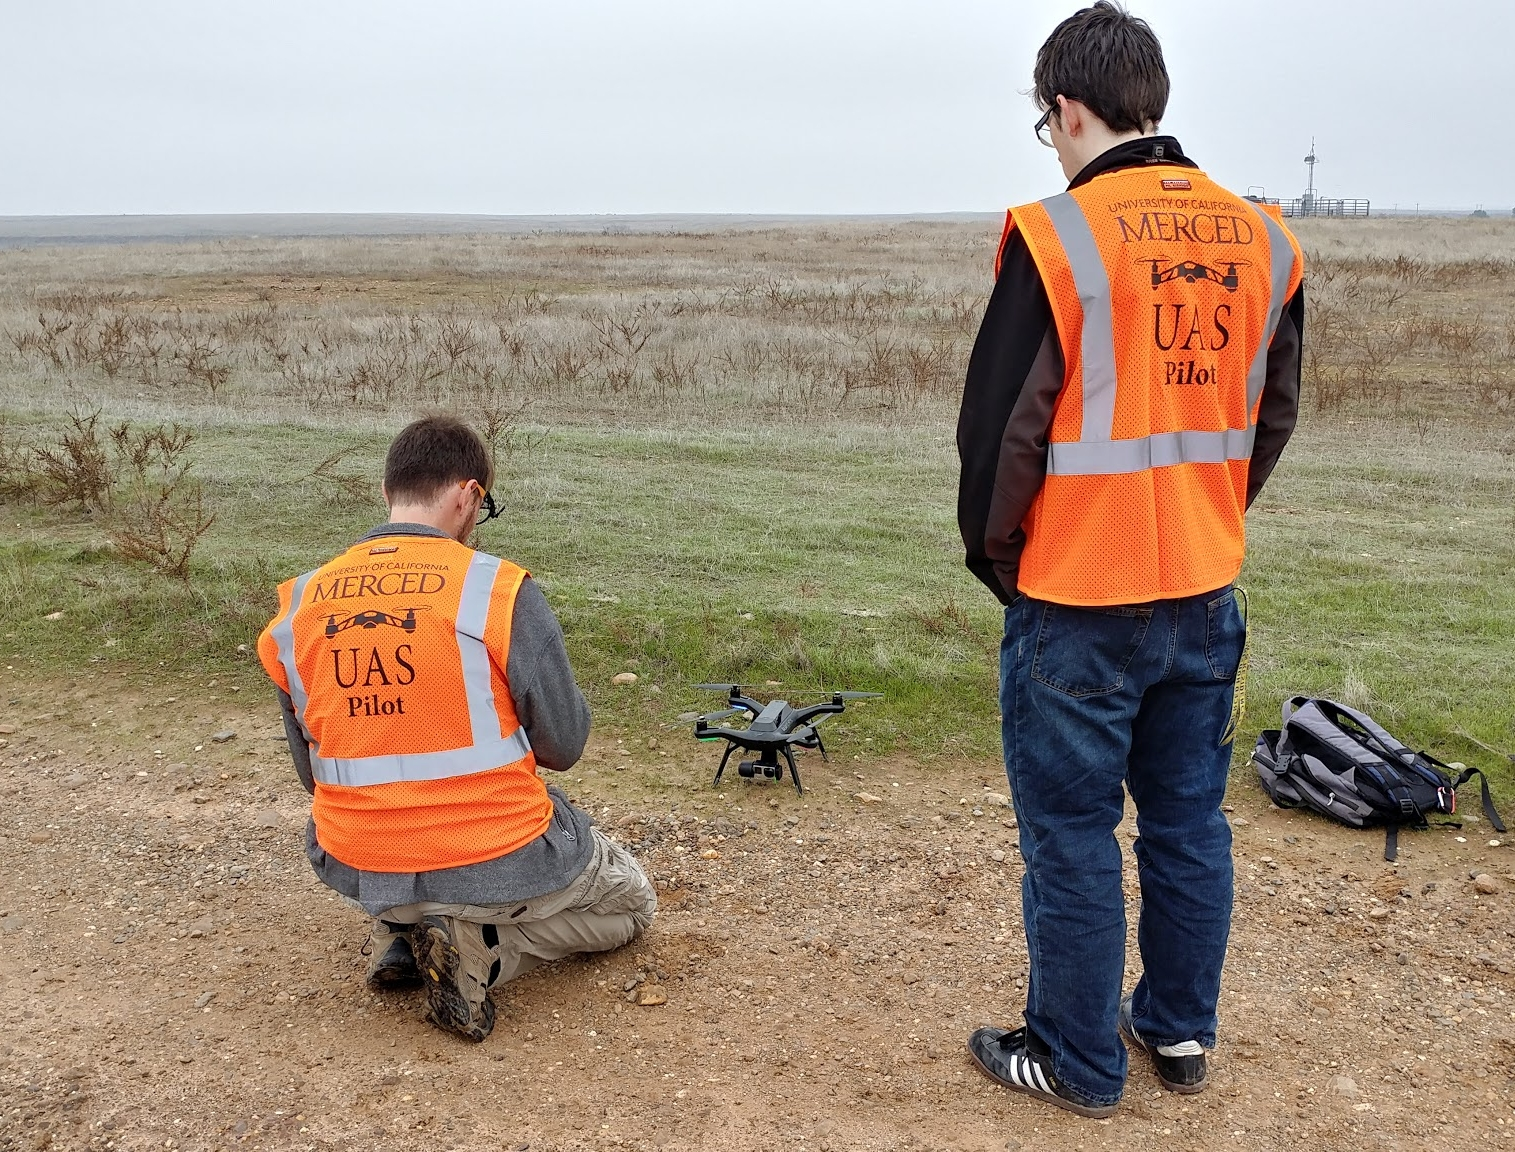
\includegraphics[width=0.75\linewidth]{images/UAS_vest} 

}

\caption{UAS operators with high visiblity vests, UC Merced}\label{fig:hivis}
\end{figure}

\hypertarget{operating-on-campus-or-other-busy-locations}{%
\section{Operating on Campus or other busy locations}\label{operating-on-campus-or-other-busy-locations}}

\begin{itemize}
\tightlist
\item
  Utilize the UC UAS Mission Planning Template (\href{http://ucdrones.github.io/library/mission_planning_template.docx}{link}) to systematically develop your flight plan
\item
  When operating in uncontrolled locations in proximity to non-participating persons, extra care should be exercised. Specific flight paths and altitudes should be pre-planned such that potential gaps in buffer or safe-zones can be identified.
\item
  High visibility vests are recommended, but not required when near nonparticipants or in public areas
\item
  Orange cones may be used to help communicate Unmanned Aircraft flight regions to non-participating persons, but are not fully sufficient.

  \begin{itemize}
  \tightlist
  \item
    Supplement any portable pedestrian control equipment (cones, caution tape, signs) with ground personnel
  \end{itemize}
\item
  If spectators are expected, a supporting ground crew member should be tasked with preventing spectators from distracting the RPIC with questions or comments.
\item
  When operating near roads, a supporting ground crew member should be tasked with being located near the road to monitor traffic, and if necessary, retrieve a fallen Unmanned Aircraft before it becomes a road hazard.
\item
  Flying above buildings and structures minimizes risk to pedestrians, but it is recommended to contact the facility manager to properly evaluate the potential risks. Some campus buildings are outfitted with research or communication equipment on rooftops.
\end{itemize}

\hypertarget{privacy-guidelines}{%
\chapter{Privacy Guidelines}\label{privacy-guidelines}}

In the United States today, the use of UAS for both recreation and commercial use are becoming ever more prominent. UAS may be used for a variety of applications, including photography and videography. The capture and use of photographs and videos from a UAS platform raises new concerns on the rights, privacies, and permissions that involve both the operators of UAS and individuals that are uninvolved in the operation. The University of California recognizes the important value of privacy and strives to achieve an appropriate balance ensuring an appropriate level of privacy, nurturing an environment of openness, honoring its obligation as a public institution to remain transparent while safe guarding information about individuals.

\textbf{Best Practices}

\begin{itemize}
\tightlist
\item
  \textbf{Do Not} use a UAS to monitor or record activities where there is a reasonable expectation of privacy.
\item
  \textbf{Do Not} use a UAS for unapproved recordings of any campus events or performances, or for any unlawful purposes.
\item
  \textbf{Do Not} fly a UAS over private property without prior approval.
\item
  \textbf{Do Not} use a UAS to harass people or intentionally disrupt events
\item
  \textbf{Do Not} use a UAS for the specific purpose of persistent and continuous collection of identifiable data about individuals without the consent of the data subjects.
\item
  \textbf{Do Not} retain identifiable data longer than reasonably necessary to fulfill a purpose.
\item
  \textbf{Do Not} knowingly publicly disclose data collected with a UAS without undertaking a reasonable effort to obfuscate or de-identify identifiable data unless the data subjects provide specific consent to the disclosure.
\item
  \textbf{Do} make a reasonable effort to provide prior notice to individuals of the general timeframe and area that they may anticipate a UAS intentionally collecting data.
\item
  \textbf{Do} establish and make available a Privacy Policy for UAS data if the UAS may intentionally or unintentionally collected identifiable data. The policy should be appropriate to the size and complexity of the data collected.
\item
  \textbf{Do} be considerate of other people's concerns over privacy, security and safety.
\item
  \textbf{Do} contact the Office of Research Compliance and Integrity if identifiable data is to be used for human-subject research.
\item
  \textbf{Do} take steps to ensure the security of any identifiable data.
\end{itemize}

\hypertarget{ch-fire-safety}{%
\chapter{Fire Safety}\label{ch-fire-safety}}

\hypertarget{fire-risk-assessment-and-planning}{%
\section{Fire Risk Assessment and Planning}\label{fire-risk-assessment-and-planning}}

\begin{itemize}
\tightlist
\item
  Assess fire risk by reviewing:

  \begin{itemize}
  \tightlist
  \item
    Calfire Red Flag Warning
  \item
    Air Quality Index (AQI)
  \item
    Vegetation levels and condition

    \begin{itemize}
    \tightlist
    \item
      Avoid operating above areas that are not viewable to monitor for fires started by a crashed UAS.
    \end{itemize}
  \end{itemize}
\item
  Equipment to bring:

  \begin{itemize}
  \tightlist
  \item
    Fire Extinguisher (ABC) for regular small fires
  \item
    Fire Extinguisher (D), or bucket of sand for LiPo fires
  \item
    Shovel (optional)
  \item
    Single-Use Fire Blankets (optional)
  \end{itemize}
\item
  Planning for the worst case:

  \begin{itemize}
  \tightlist
  \item
    Ensure that emergency communication systems are always available during flight operations.
  \item
    Ensure that all flight crew members can describe the flight operation location and how to get to the site to emergency personnel
  \item
    Ensure that all PPE is appropriate for the operation
  \end{itemize}
\end{itemize}

\hypertarget{battery-fire}{%
\section{Battery Fire}\label{battery-fire}}

\begin{itemize}
\tightlist
\item
  Secure the site.
\item
  Remove any other potential fire fuel or other fire hazards.
\item
  Use a Class ABC fire extinguisher to extinguish and control any secondary fires.
\item
  Use a Class D fire extinguisher or a bucket of sand to extinguish the fire at the battery itself.
\item
  Avoid using water - if no other option, submerge the entire battery in water.
\item
  If you are unable to extinguish the fire:

  \begin{itemize}
  \tightlist
  \item
    Call emergency services
  \item
    Stop all fire suppression efforts and begin minimizing potential damage by clearing the area and removing other potential fire hazards
  \end{itemize}
\item
  DO NOT COMPROMISE YOUR SAFETY
\end{itemize}

\hypertarget{in-flight-or-post-flight-fire}{%
\section{In-Flight or Post-Flight Fire}\label{in-flight-or-post-flight-fire}}

\begin{itemize}
\tightlist
\item
  Maintain visual contact with UAS
\item
  Communicate the situation to the Flight Crew
\item
  Verify

  \begin{itemize}
  \tightlist
  \item
    Check state of UAS (Status/Flight Mode)
  \item
    Check UAS location/altitude
  \item
    Check transmitter/tablet status and control links
  \end{itemize}
\item
  Take Actions

  \begin{itemize}
  \tightlist
  \item
    Ground Crew -- Alert and clear flight area, prepare safety equipment
  \item
    Visual Observer -- Be prepared to call emergency services
  \item
    RPIC -- Immediately terminate flight
  \end{itemize}
\item
  Issues

  \begin{itemize}
  \tightlist
  \item
    If UAS sparks a ground fire:

    \begin{itemize}
    \tightlist
    \item
      Secure site and attempt to extinguish the fire with Ground Crew
    \end{itemize}
  \item
    If unable to extinguish fire:

    \begin{itemize}
    \tightlist
    \item
      Call emergency services
    \item
      Stop all fire suppression efforts and begin minimizing potential damage by clearing the area and removing other potential fire hazards
    \end{itemize}
  \item
    DO NOT COMPROMISE YOUR SAFETY
  \end{itemize}
\item
  Post-Incident

  \begin{itemize}
  \tightlist
  \item
    Document incident
  \item
    Contact campus designated local authority or systemwide designated UAS authority
  \end{itemize}
\end{itemize}

\hypertarget{ch-cold-weather}{%
\chapter{Operations in Cold Weather}\label{ch-cold-weather}}

\hypertarget{cold-environments}{%
\section{Cold Environments}\label{cold-environments}}

\begin{itemize}
\tightlist
\item
  Before beginning flight operations, double check the weather conditions. Avoid starting flight operations if there is potential for a shift in weather conditions, such as incoming strong winds, rain, and snow.
\item
  Do not fly in temperatures below \(0^\circ\)C (\(32^\circ\)F).
\item
  Avoid contact with snow. Moisture can damage the motors. Use a large landing pad for taking off and landing your UAS.
\item
  Expect to see a 10-15\% decrease in flight time - plan missions accordingly.
\end{itemize}

\hypertarget{cold-battery}{%
\section{Battery Considerations}\label{cold-battery}}

\begin{itemize}
\tightlist
\item
  Only use fully charged batteries.
\item
  Pre-warm batteries to \(20^\circ\)C (\(68^\circ\)F) or more.
\item
  Check the battery temperature in DJI GO.
\item
  Use an insulated cooler, or keep in a warm car to maintain temperature when not in use.
\item
  After launching, hover for about a minute to allow the battery to warm up.
\item
  Avoid aggressive flight maneuvers and land flights earlier than in normal weather.
\item
  Batteries drain faster in cold temperatures. Always check the UAS battery status during flight.
\end{itemize}

\hypertarget{ch-hot_weather}{%
\chapter{Operations in Hot Weather}\label{ch-hot_weather}}

\hypertarget{hot-environments}{%
\section{Hot Environments}\label{hot-environments}}

\begin{itemize}
\tightlist
\item
  Try to avoid flight operations in extreme heat or humidity levels.
\item
  Do not fly in temperatures above \(110^\circ\)C (\(43^\circ\)F).
\item
  Keep flights to short bursts, and rest the UAS in the shade between flight operations.
\item
  Monitor the controller and tablet temperature. Avoid direct sunlight.
\item
  If possible, try to operate under shade or a small canopy.
\item
  Expect to see a 10-15\% decrease in flight time - plan missions accordingly.
\end{itemize}

\hypertarget{hot-battery}{%
\section{Battery Considerations}\label{hot-battery}}

\begin{itemize}
\tightlist
\item
  Only use fully charged batteries.
\item
  Never use batteries that are abnormally hot to the touch.
\item
  Check the battery temperature in DJI GO.
\item
  Use an insulated cooler and keep in the shade to keep cool when not in use.
\item
  Avoid aggressive flight maneuvers and land flights earlier than in normal weather.
\item
  Batteries drain faster in hot temperatures. Always check the UAS battery status during flight.
\item
  Never leave a battery in direct sunlight
\item
  After use, store the depleted battery in a well-ventilated area to allow it to cooldown. Do not place in a storage case or bag.
\end{itemize}

\hypertarget{ch-battery-care}{%
\chapter*{Battery Care Guidance}\label{ch-battery-care}}
\addcontentsline{toc}{chapter}{Battery Care Guidance}

\textbf{Lithium Polymer batteries have a limited lifespan and should be replaced as necessary}

\hypertarget{battery-maintenance}{%
\section{Battery Maintenance}\label{battery-maintenance}}

\begin{itemize}
\tightlist
\item
  Aim to keep battery levels above 40\% and below 65\% when not in use.
\item
  Avoid charging the batteries to max capacity unless you are going to fly within the next day.
\item
  When done flying, always charge your batteries at least back up to storage level (40\%).
\item
  Remove batteries from the aircraft when stored for an extended period.
\item
  Never over-discharge your battery.
\item
  Fully charge and discharge the battery at least once every 3 months to maintain battery health
\item
  Do not place loose batteries on any conductive surfaces, such as metal tables.
\item
  Batteries must be stored in climate controlled storage when not in use. Do not expose to excessive heat or humidity.
\end{itemize}

\hypertarget{preparing-for-flight}{%
\section{Preparing for flight}\label{preparing-for-flight}}

\begin{itemize}
\tightlist
\item
  When charging batteries, ensure that the charging location is clean, uncluttered and well-ventilated.
\item
  Do not stack chargers when charging batteries, or place batteries on the power adapter during charging.
\item
  Do not leave batteries charging unattended.
\item
  Do not charge batteries near flammable materials or on flammable surfaces.
\item
  Plan to charge batteries no earlier than 3 days prior to flight.
\end{itemize}

\hypertarget{immediately-after-flight}{%
\section{Immediately after flight}\label{immediately-after-flight}}

\begin{itemize}
\tightlist
\item
  Power off the aircraft completely before removing the battery.
\item
  After removing a used battery, store the battery in a shaded, but well-ventilated location.\\
\item
  Never store a recently used and warm battery in an enclosed battery bag or UAS case.
\item
  Document any performance issues immediately.
\end{itemize}

\hypertarget{battery-inspection}{%
\section{Battery Inspection}\label{battery-inspection}}

\begin{itemize}
\tightlist
\item
  Check battery voltage levels at least once a month when not in use.
\item
  Check for bulging, swelling or cracks in battery casing.
\item
  Check for signs of electrical arcing, such as burn marks or melted plastic around the battery terminals.
\item
  Safely discard any battery that is showing any sign of damage or bulging.
\end{itemize}

\hypertarget{battery-travel}{%
\section{Battery Travel}\label{battery-travel}}

\begin{itemize}
\tightlist
\item
  Always store batteries in a ventilated location
\item
  Never transport a damaged battery or a battery with less than 5\% remaining
\item
  Always store batteries in a specified transportation box/bag before the transit to avoid damage from external forces.
\item
  Do not store a battery with metal components such as paperclips, screws or metal nuts.
\end{itemize}

\hypertarget{battery-incidents}{%
\section{Battery Incidents}\label{battery-incidents}}

\begin{itemize}
\tightlist
\item
  Do not use a battery that has been involved in a serious crash or heavy impact.
\item
  If a battery falls into water with the aircraft during flight, take it out immediately, and place it in a safe and open area. Maintain a safe distance from the battery until it is completely dry. Never use the battery again, and dispose of the battery properly. Do not use heat to dry batteries.\\
\item
  Put out any battery fire using sand, or a dry powder fire extinguisher.
\end{itemize}

\hypertarget{part-mission-documentation}{%
\part{Mission Documentation}\label{part-mission-documentation}}

\hypertarget{uc-drones-project-or-flight-request}{%
\chapter{UC Drones Project or Flight Request}\label{uc-drones-project-or-flight-request}}

\textbf{Place a copy or link to your UC Drones Project or Flight Request here}

\begin{itemize}
\tightlist
\item
  Do not forget to include your mission plan and hazard analysis if it is attached as a separate file
\end{itemize}

\hypertarget{ch-weather}{%
\chapter{Weather Forecast}\label{ch-weather}}

**Place a copy of link to the weather forecast during your flight operations

\hypertarget{ch-airspace}{%
\chapter{Airspace Information}\label{ch-airspace}}

\textbf{Document any airspace issues including}

\begin{itemize}
\tightlist
\item
  Airspace Class
\item
  Nearby airports and heliports
\item
  Small landing strips, glider ports and sea ports
\item
  Areas of potential aviation activities - crop dusting, helicopter tours, VFR checkpoints
\end{itemize}

\textbf{Look for and Review any NOTAMS and TFRs within your operating area}

\hypertarget{ch-performance-log}{%
\chapter{Log of Recent UAS performance}\label{ch-performance-log}}

\textbf{Draft a review of the recent UAS performance and any relevant notes that may be useful to communicate during the preflight briefing.}

\hypertarget{ch-emergency}{%
\chapter{Emergency Contact Information}\label{ch-emergency}}

\hypertarget{uc-center-of-excellence-on-uas-safety}{%
\section{UC Center of Excellence on UAS Safety}\label{uc-center-of-excellence-on-uas-safety}}

\textbf{Contact Information}

\begin{verbatim}
Dr. Brandon Stark
(209) 201-2051
bstark2@ucmerced.edu
UASsafety@ucmerced.edu
\end{verbatim}

\hypertarget{campus-designated-local-authority}{%
\section{Campus Designated Local Authority}\label{campus-designated-local-authority}}

\textbf{Campus}

\begin{center}\rule{0.5\linewidth}{0.5pt}\end{center}

\textbf{Contact information for Campus Point of Contact}

\begin{center}\rule{0.5\linewidth}{0.5pt}\end{center}

List of Campus Point of Contact can be found here: \url{https://ucdrones.github.io/ch-DLA.html}

\hypertarget{nearest-emergency-facility}{%
\section{Nearest Emergency Facility}\label{nearest-emergency-facility}}

\textbf{Enter Contact information for the nearest emergency facility}

\hypertarget{uas-operation-site}{%
\section{UAS Operation Site}\label{uas-operation-site}}

\textbf{Address of UAS Operation Site}

\textbf{Write out directions on how to get to the site from the nearest crossroad}

\hypertarget{part-other-documentation}{%
\part{Other Documentation}\label{part-other-documentation}}

\hypertarget{remote-pilot-certificate}{%
\chapter{Remote Pilot Certificate}\label{remote-pilot-certificate}}

\textbf{Place a copy of your Remote Pilot Certificate Here }

\hypertarget{airspace-or-waiver-documentation}{%
\chapter{Airspace or Waiver Documentation}\label{airspace-or-waiver-documentation}}

\textbf{Append with any Airspace or Waiver Documentation}

  \bibliography{book.bib,packages.bib}

\end{document}
